\section{Diseño}
A continuación se presentan y explican algunas de las desiciones de diseño elegidas durante el desarrollo del trabajo practico.
Se decidió dividir la presentación en subsecciones para facilitar la comprensión de la misma, haciendo especial enfasis en aquellas que sentiamos eran de importancia para la comprensión del mismo.

Vale mencionar que si bien es cierto que se genero una idea general en el grupo antes de comenzar a reflejar las decisiones tomadas en codigo, el diseño en profundidad se termino de desarrollar y afinar en paralelo, mientras surgian cuestiones mismas relacionadas al propio desarrollo que no habian sido tenidas en cuenta en papel. 

\subsection{Acciones}
Todas las jugadas que pueden desarrollarse durante la simulacion de un partido, se divide claramente en dos grupos. Aquellas que realiza el equipo que esta atacando, y aquellas que realiza aquel que esta defendiendo. En base a esta idea, planteamos nuestro diseño clasificando a todas las acciones que pueden realizarse dentro de una jugada, en alguno de estos dos grupos (Ofensivas y Defensivas) y sub clasificando luego, de acuerdo al tipo de accion.
Este diseño, ademas de presentar de forma simple la realidad, nos permite extender el modelo con nuevas acciones tanto ofensivas como defensivas, de manera relativamente sencilla. Bastaria simplemente con declarar una nueva clase de herede de el tipo de clasificacion correspondiente de la accion. Por supuesto, la accion conoce al jugador que la esta ejecutando para poder mantener la informacion de la simulación de forma consistente.
\begin{center}
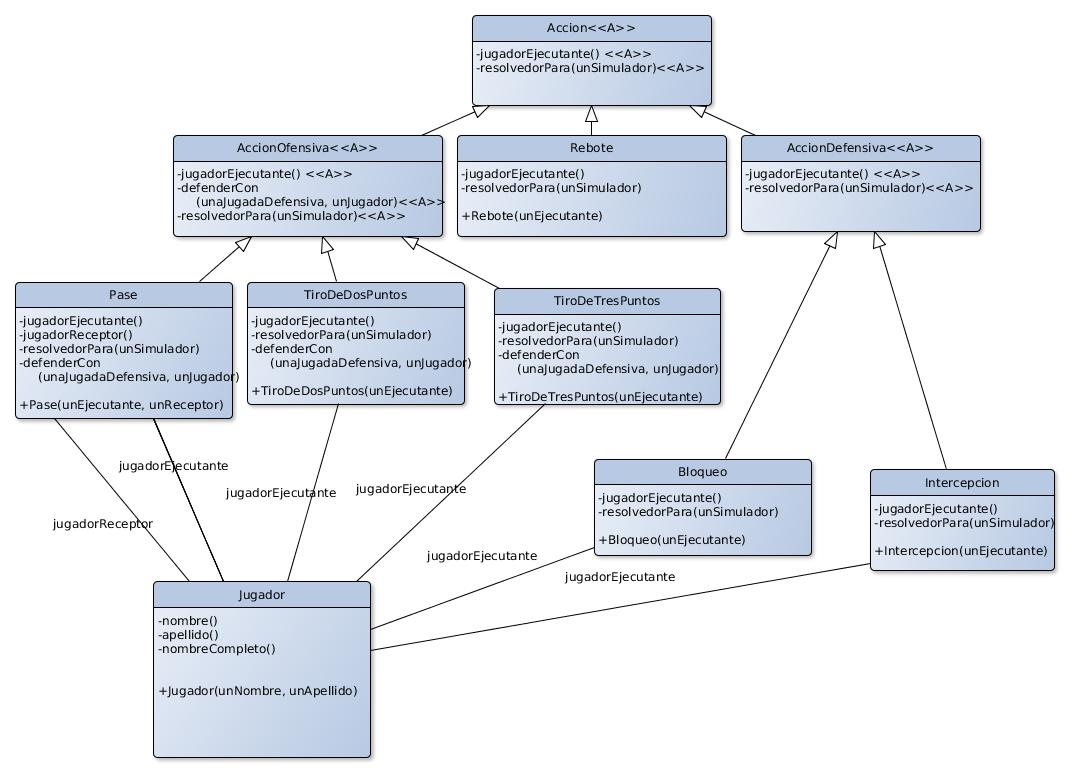
\includegraphics[scale=0.35]{diseno/acciones.jpg}
\end{center}

\subsection{Jugadas y acciones}
A continuación, presentamos entonces, como es que cada una de las acciones mencionadas en el apartado anterior, se integra con las jugadas defensivas/ofensivas, que componen los libros de los tecnicos.
\begin{center}
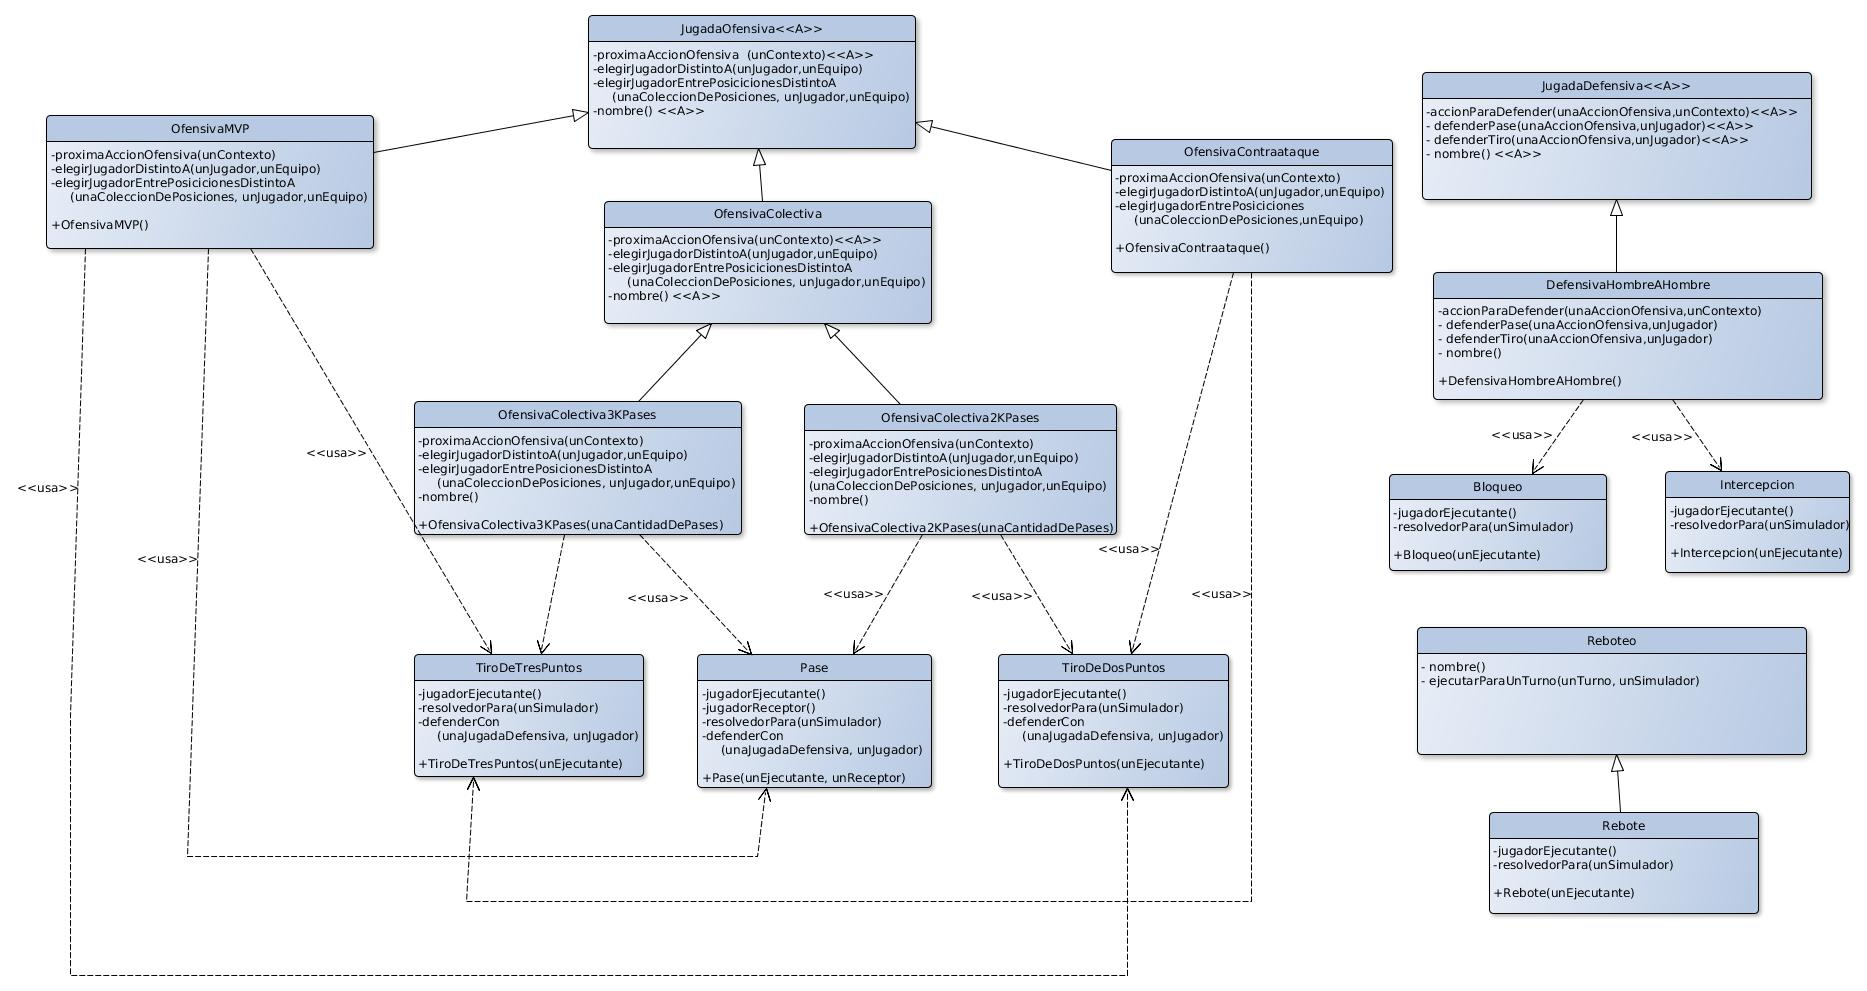
\includegraphics[scale=0.4, angle=90]{diseno/jugadasYAcciones.jpg}
\end{center}


\subsection{Apuestas}
Decidimos que la mejor forma de clasificar las apuestas era mediante una jerarquizacion, para poder representar de forma clara que existen aquellas en las que se pone en juego un numero X de fichas, pero tambien aquellas nulas en las que no hay cap apostado. Esta clasificación, si bien es posible que agregue mas complejidad al diseño que suponiendo que las apuestas nulas son aquellas con cantidad de fichas igual a cero, nos ahorra de tener que manejar un unico tipo de apuesta y preguntar por la cantidad de fichas apostados todo el tiempo, permitiendo alijerar el manejo de las apuestas.
\begin{center}
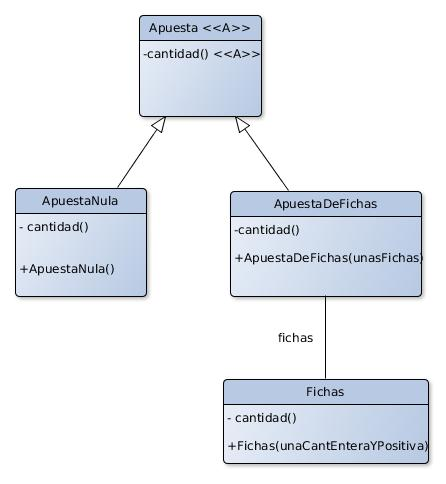
\includegraphics[scale=0.4]{diseno/apuestas.jpg}
\end{center}

\subsection{Equipo, jugadores y tecnico}
Para modelar al equipo, decidimos que exista una clase abstracta posición donde se hereden cada una de las posibles posiciones que puede adoptar un jugador. Nos parecio que es la forma mas correcta de representar la realidad, y si bien es cierto que en el tiempo las posibles posiciones no vayan a variar, nos permite diferenciar a cada jugador de manera sencilla a la hora de saber su interaccion dentro de una jugada. El tecnico, a su vez, cuenta con un libro de jugadas que puede usar tanto ofensivas como defensivas. Una forma simple de representar y distinguir ambas formas de juego.
\begin{center}
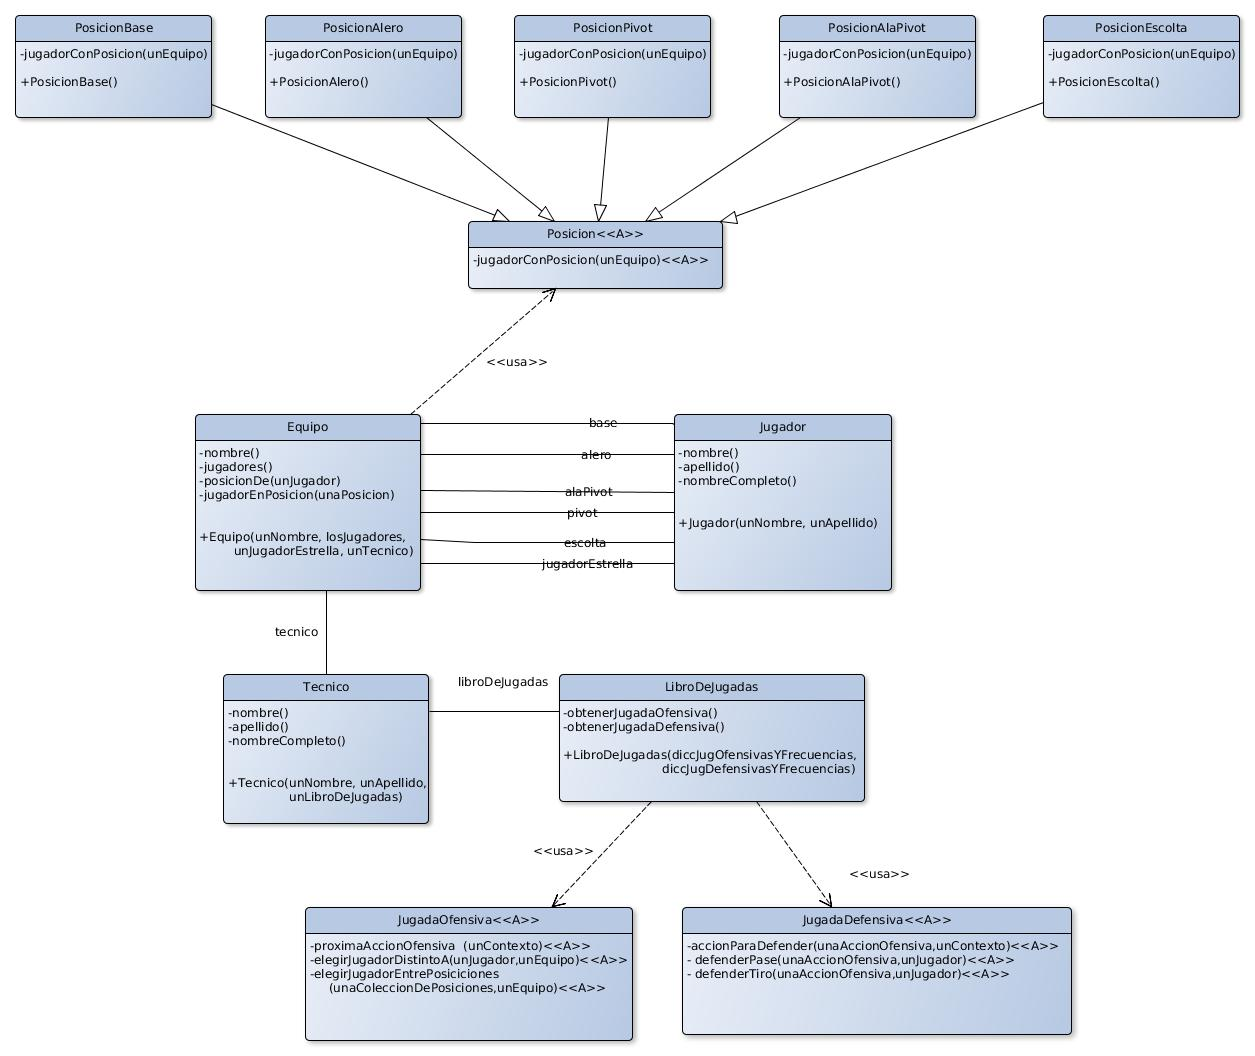
\includegraphics[scale=0.4]{diseno/equipo.jpg} 
\end{center}

\subsection{Gestor de Equipos}
El gesto de equipos es aquel encargado de dar de alta y realizar cada una de las validaciones necesarias para confirmar la creacion de un equipo. Es por eso que se necesita de un gestor de Cap y una entidad que represente una lista de cada uno de los posibles jugadores. Esta elección nos permite disminuir la cohesión del modelo, permitiendo asi que futuras validaciones o modificaciones a las ya existentes, se agreguen de forma simple y sin agregar complejidad.
\begin{center}
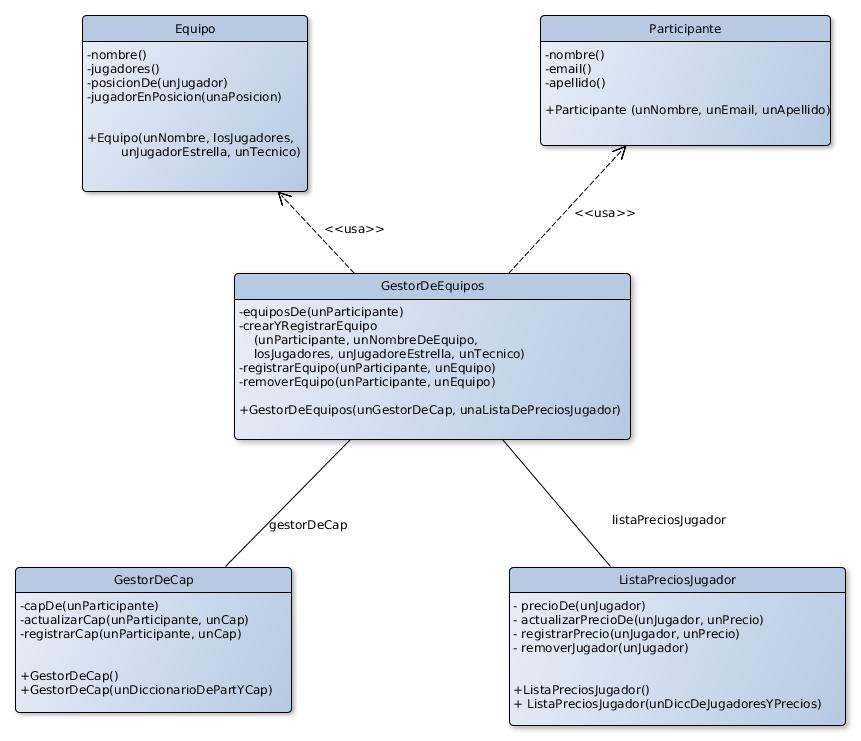
\includegraphics[scale=0.4]{diseno/gestorDeEquipos.jpg}
\end{center}

\subsection{Gestor de Cap y Fichas}
Estas dos entidades usan la misma logica y, conociendo al participante y la entidad a gestionar, permiten registrar y actualizar el cap y la cantidad de fichas de los participantes
\begin{center}
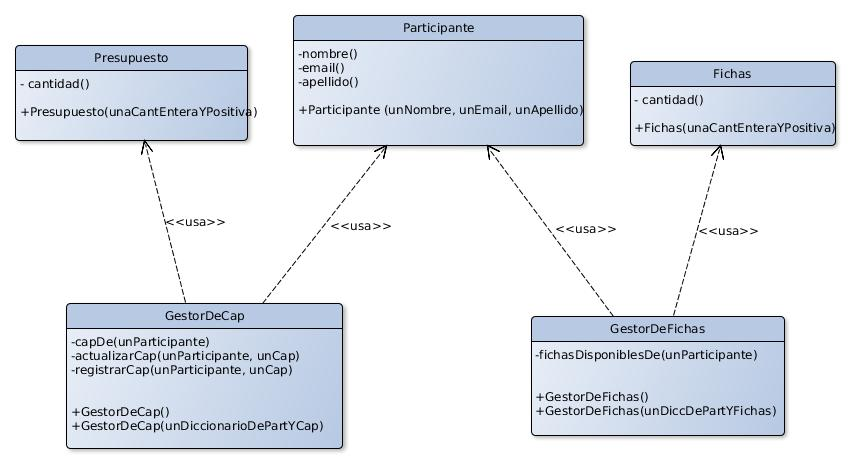
\includegraphics[scale=0.4]{diseno/gestorDeCapYFichas.jpg} 
\end{center}

\subsection{Registro de estadisticas}
Por ultimo, decidimos contar con una entidad encargada de llevar un registro de las estadisticas de cada uno de los jugadores porque no tenia sentido que un jugador sepa responder sus estadisticas. Esto nos permitia modelar la realidad de forma mas fehaciente, dejando abierta la posibilidad de cambios en las estadisticas de forma limpia para el futuro.
\begin{center}
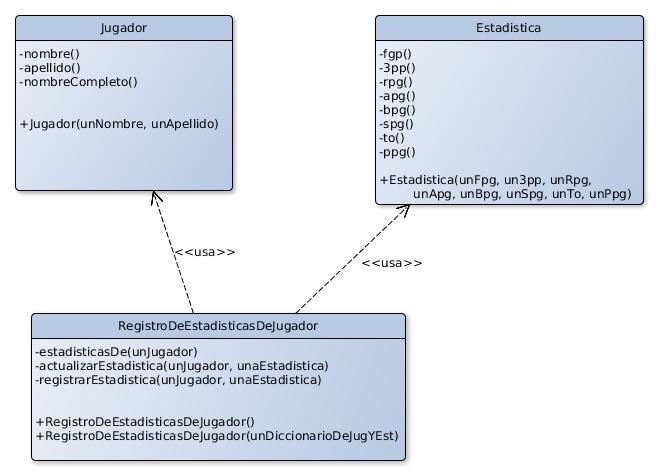
\includegraphics[scale=0.4]{diseno/registroDeEstadisticas.jpg}
\end{center}

